%%%%%%%%%%%%%%%%%%%%%%%%%%%%%%%%%%%%%%%%%%%%%%%%%%%%%%%%%%%%%%%%%%%%%%%%%%%%%%
\section{Relative tracker-calorimeter timing offset}

In an event which has a calorimeter cluster matching to a reconstructed track, the
cluster is included into the track fit as an additional hit. The algorithm reconstructing 
straw hits in the tracker and the algorithm reconstructing the waveform timing in the calorimeter
could add different timing offsets to the reconstructed hist and clusters correspondingly.
Those offsets need to be calibrated out.

A cluster is included into the track fit with the coordinate error $\sigma_{XY} = 15$ mm
and the timing error $\sigma_T = 0.5ns$.

The distribution of the calorimeter cluster timing residuals for conversion electrons
is shown in Figure \ref{fig:track_cluster_dt_default}

\begin{figure}
\begin{tikzpicture}
  \node[anchor=south west,inner sep=0] at (0,0.) {
    % \node[shift={(0 cm,0.cm)},inner sep=0,rotate={90}] at (0,0) {}
    \makebox[\textwidth][c] {
      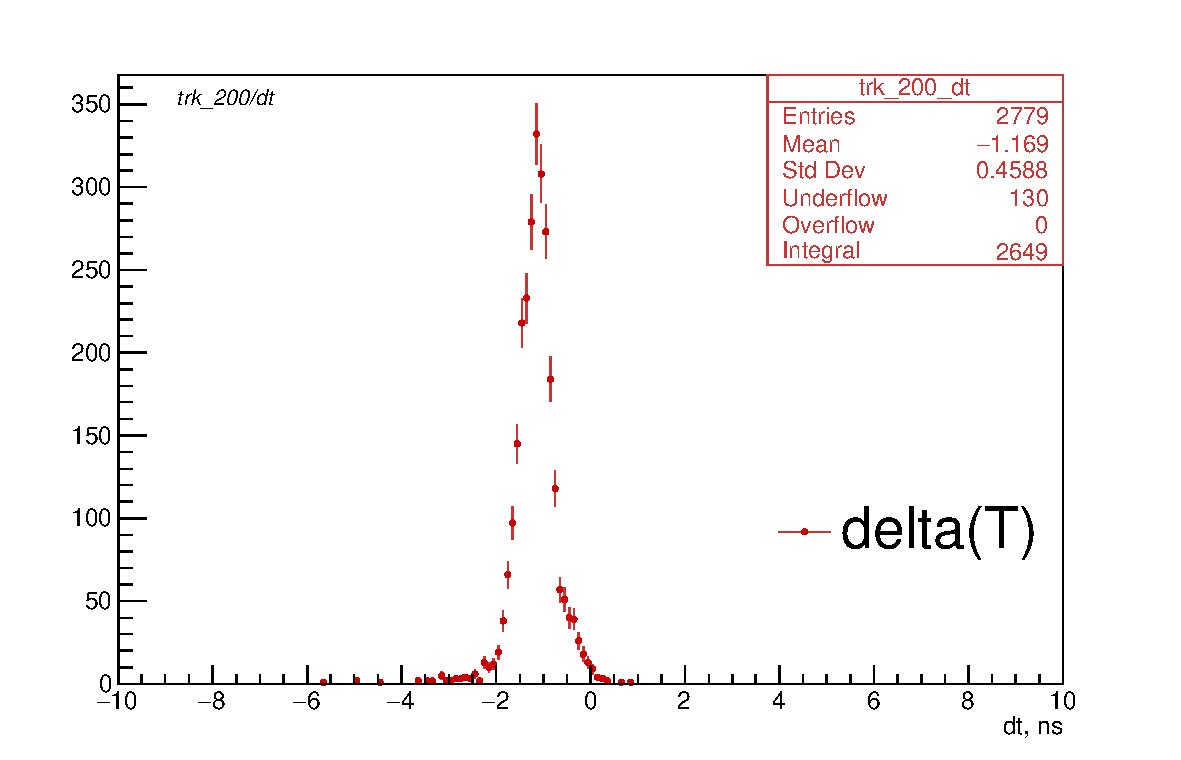
\includegraphics[width=0.99\textwidth]{figures/pdf/figure_00001_ele00_05_15_su2020_track_ana_par}
    }
  };
  % \node [text width=6cm, scale=0.8] at (4.5,6.4) {mu2e-18894 by Kevin Lynch and Jim Popp};
\end{tikzpicture}
% \captionof{figure} {
\caption{
  \label{fig:track_cluster_dt_default}
  track-cluster timing residuals
}
\end{figure}

%%% Local Variables:
%%% mode: latex
%%% TeX-master: "mu2e-36375"
%%% End:
